\begin{frame}{From physics to the mathematical model}
  \vspace{-0.6cm}
  \begin{overprint}
    \onslide<1>
    \begin{columns}
      \begin{column}{0.45\textwidth}
        \begin{block}{Solid dynamics problems}
          \begin{itemize}
          \item[] \textbf{Impact; Crash-proof design}
          \item[] High-speed forming
          \item[] Earthquake reliability of structures 
          \end{itemize}
        \end{block}
      \end{column}
      
      \begin{column}{0.55\textwidth}
      \end{column}
    \end{columns}
    
    \begin{figure}[ht]
      \centering
      \subcaptionbox{Bird strike on aircrafts}{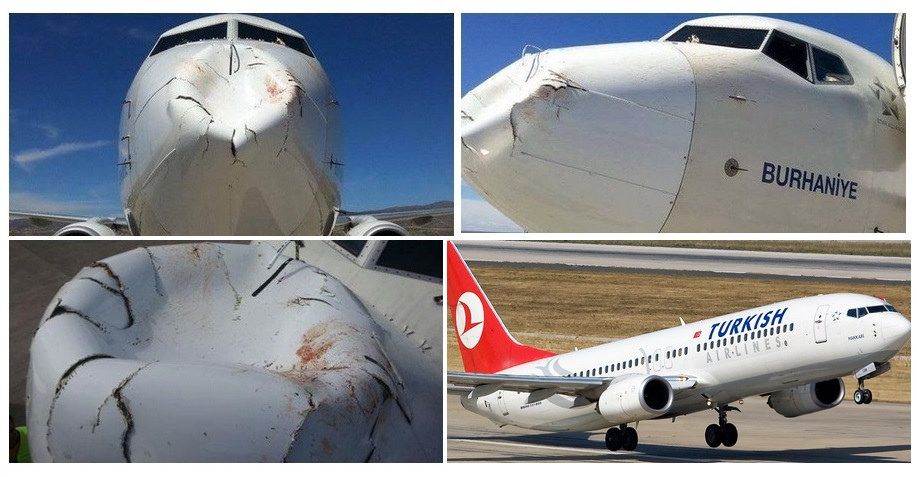
\includegraphics[height=0.3\paperheight]{section1/pictures/birdstrike.jpg}}
      \subcaptionbox{Glasgow Museum of Transport}{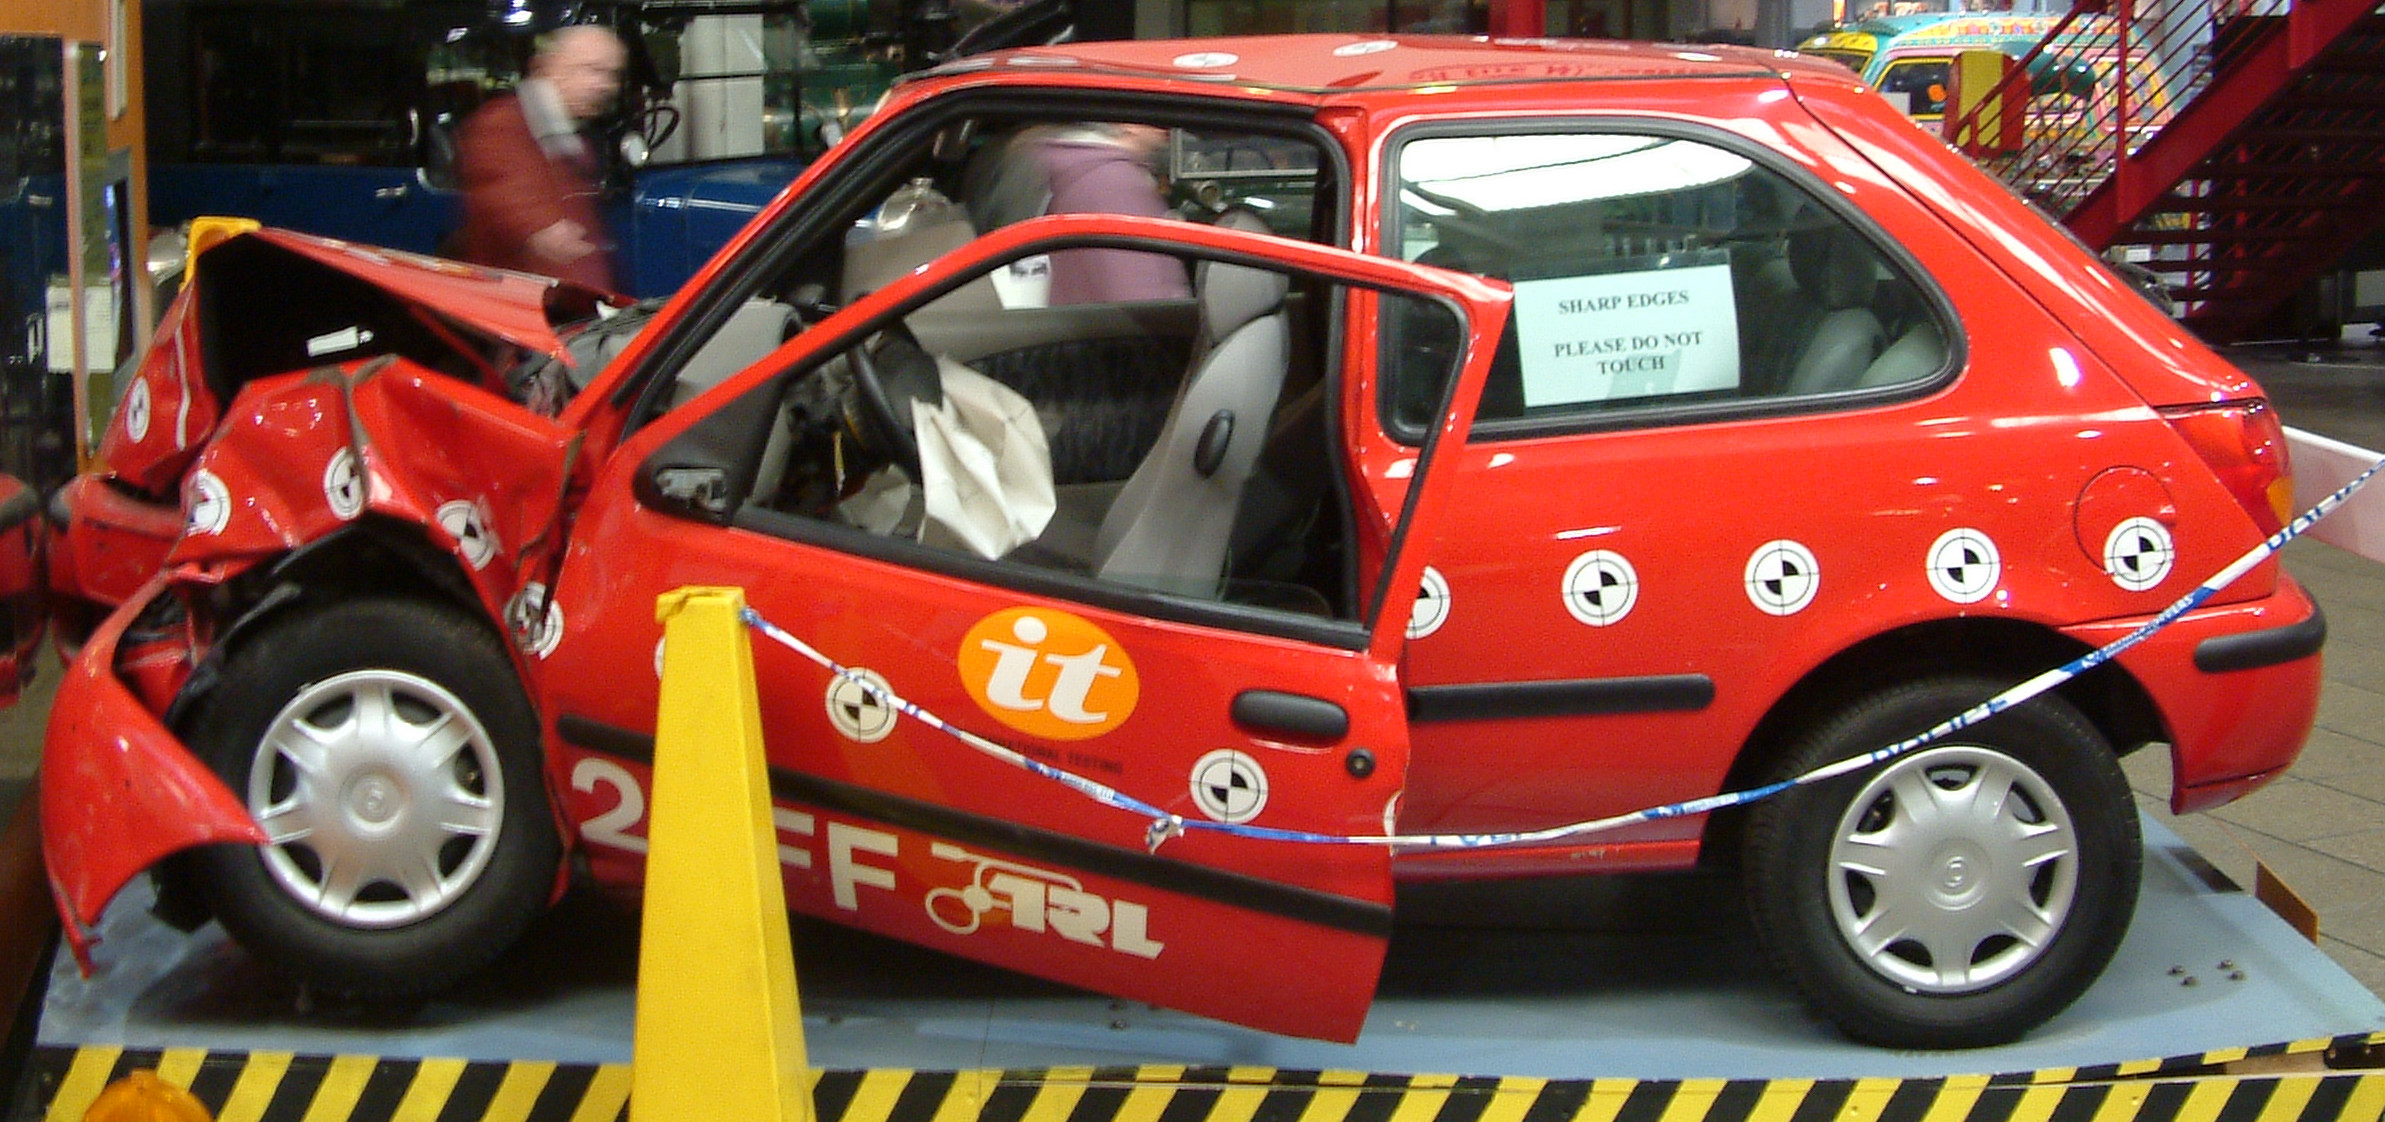
\includegraphics[height=0.3\paperheight]{section1/pictures/crash2.jpg}}
    \end{figure}
    
    \onslide<2>
    \begin{columns}
      \begin{column}{0.45\textwidth}
        \begin{block}{Solid dynamics problems}
          \begin{itemize}
          \item[] Impact; Crash-proof design
          \item[] \textbf{High-speed forming}
          \item[] Earthquake reliability of structures 
          \end{itemize}
        \end{block}
      \end{column}
      
      \begin{column}{0.55\textwidth}
      \end{column}
    \end{columns}
    \centering
      \movie[height = 0.35\paperheight,width=0.25\linewidth,loop,poster,autostart]{}{%
      section1/animation/output3.mp4}\\
    \scriptsize Electromagnetic forming \cite{Guillaume}
    \footnoteCite{Guillaume}
    
    % \vfill
    % {\tiny
    %   \usebibitemtemplate{\color{structure}\insertbiblabel} 
    %   \usebibliographyblocktemplate{\color{structure}}{\color{black}}{\color{structure!75}}{\color{structure!75}} 
    %   \begin{thebibliography}{EMF}
    %     \tiny \bibitem[1]{Formage}
    %     Bon E.,Priem D.,Sow C., Heuzé T., Racineux G.
    %     \newblock Electromagnetic bending of an aluminum sheet
    %     \newblock {\em GeM, Ecole centrale de Nantes, 2015}.
    %   \end{thebibliography}}
    

    \onslide<3>
    \begin{columns}
      \begin{column}{0.45\textwidth}
        \begin{block}{Solid dynamics problems}
          \begin{itemize}
          \item[] Impact; Crash-proof design
          \item[] High-speed forming
          \item[] \textbf{Earthquake reliability of structures}
          \end{itemize}
        \end{block}
      \end{column}
      
      \begin{column}{0.55\textwidth}
      \end{column}
    \end{columns}

    \centering
    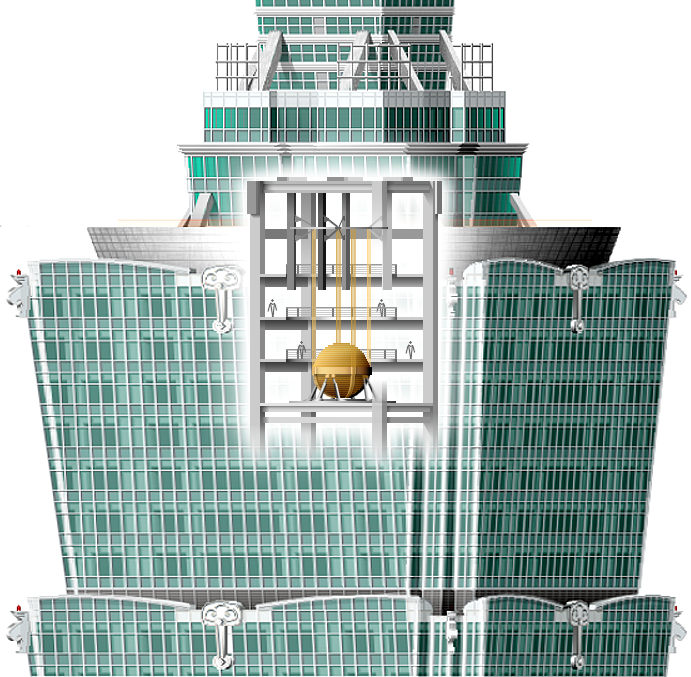
\includegraphics[scale=0.15]{section1/pictures/TaipeiTower.png} \quad
    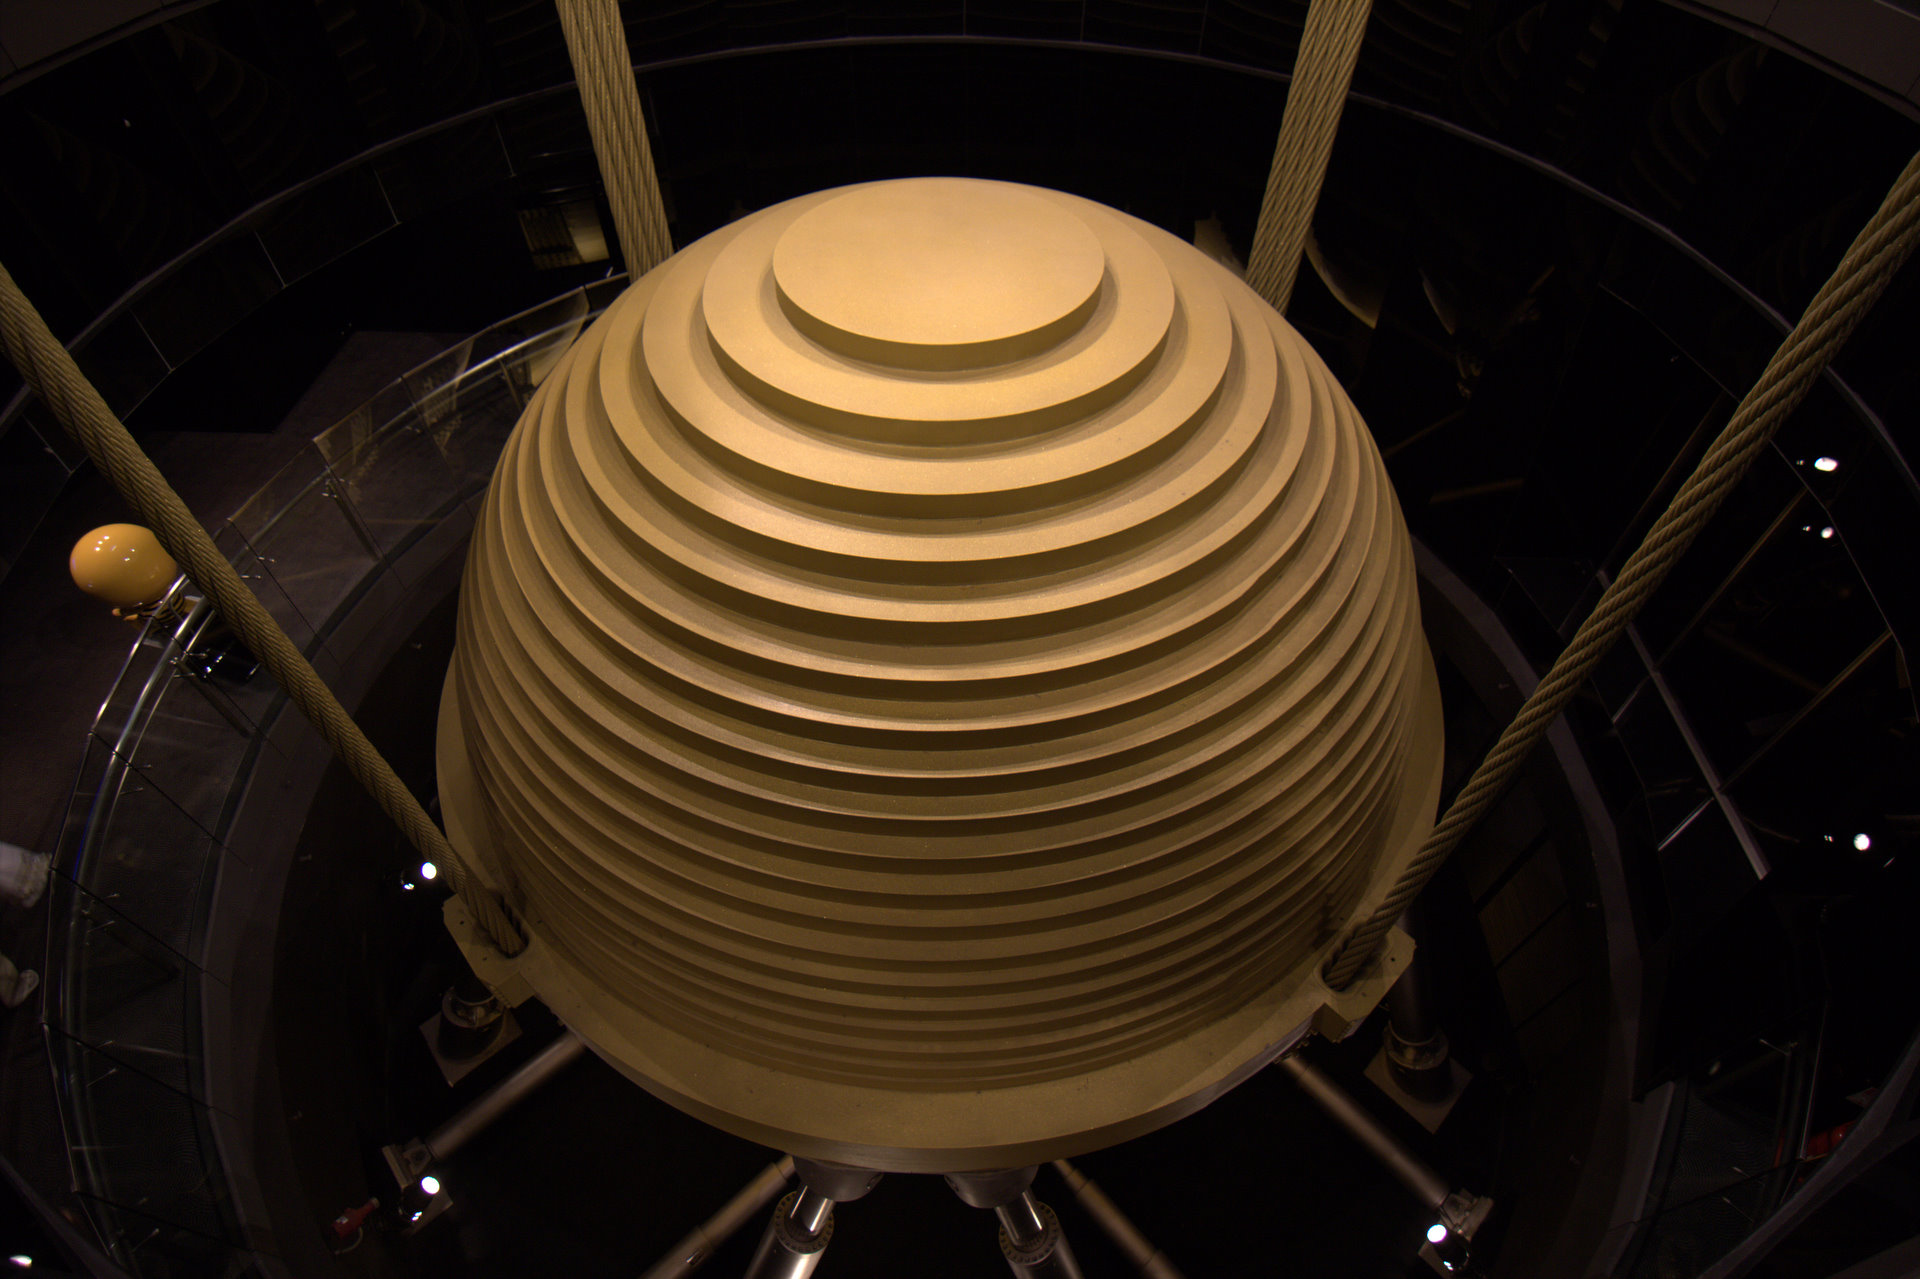
\includegraphics[scale=0.08]{section1/pictures/MassDamper.jpg}\\
    \scriptsize Taipei 101 mass damper

    \onslide<4>
    \begin{columns}
      \begin{column}{0.45\textwidth}
        \begin{block}{Solid dynamics problems}
          \begin{itemize}
          \item[] Impact; Crash-proof design
          \item[] High-speed forming
          \item[] Earthquake reliability of structures 
          \end{itemize}
        \end{block}
      \end{column}
      
      \begin{column}{0.55\textwidth}
        \begin{block}{Partial differential equations}
          \begin{equation*}
            \Rightarrow \left\lvert
              \begin{aligned}
                & \text{Conservation laws} \\
                & \text{Constitutive equations} 
              \end{aligned}
            \right. = \textbf{Hyperbolic system}
            % Préciser les équations dans le dévelopement de la DGMPM
          \end{equation*}
        \end{block}
      \end{column}
    \end{columns}
    
    \begin{block}{Difficulties for the solution of hyperbolic equations:}
      \begin{itemize}
      \item complex geometries
      \item waves propagating/interacting in solids \cite{Wang}
      \item finite deformations
      \end{itemize}
    \end{block}
    \textbf{$\Rightarrow$ Resort to numerical simulation:} space and time discretization techniques
    \footnoteCite{Wang}
  \end{overprint}
  
\end{frame}

% Problems considered -- dynamics + applications + solid mechanics (equations)
% Soit (i) on inclue les équations du modèle dans les motivations soit (ii) on parle d'abord des difficultés qu'après on illustre ?

% (i) - Problèmes de dynamique des solides: lois de conservations + lois constitutives => système hyperbolique
% - EDP dont les solutions font intervenir des ondes
% - Equations complexes (non-linéaires + multi-dimensionnelle) + solutions compliquées car ondes qui interagissent
% - Intérêt de la simulation pour calculer des solutions approchées
% - Mais cependant, on a des limitations (grandes defs ; suivi des ondes [oscillations + diffusion] ; difficultées à assurer la convergence vers une solution physique ??? [un truc pour introduire la prise en compte de la structure caractéristique])
% - Exemples de limitations avec les méthodes existantes : FEM -- FV -- Meshfree 

\begin{frame}{Suitability of some explicit methods}
  \begin{block}{The Finite Element Method \cite{Belytschko}}
    \vskip 4pt
    \begin{overprint}
      \onslide<1>
      \begin{columns}
        \begin{footnotesize}
          \begin{column}{0.5\textwidth}
            \begin{itemize}
            \item[] Mesh-based space discretization
            \item[] Weak form of balance equation
            \end{itemize}
          \end{column}
          \begin{column}{0.5\textwidth} 
            \begin{itemize}
            \item[] Polynomial approximation
            \item[] Gauss points constitutive update
            \end{itemize}
          \end{column}
        \end{footnotesize}
      \end{columns}
      \onslide<2>
      \begin{columns}
        \begin{footnotesize}
          \begin{column}{0.5\textwidth}
            \begin{itemize}
            \item[] Mesh-based space discretization
            \item[] Weak form of balance equation
            \end{itemize}
          \end{column}
          \begin{column}{0.5\textwidth} 
            \begin{itemize}
            \item[] Polynomial approximation
            \item[] Gauss points constitutive update
            \end{itemize}
          \end{column}
        \end{footnotesize}
      \end{columns}
      \vskip -10pt
      \begin{columns}
        \begin{column}{0.48\textwidth}
          \begin{block}{\footnotesize Lagrangian formulation}
            \centering
            \begin{tikzpicture}[scale=0.4]
              \tkzKiviatDiagram[lattice=4,
              label style/.append style={font=\scriptsize},radial  style/.style ={->},lattice style/.style ={white,opacity=0}]{CFL,Non-diffusive,Distortion-free,Non-oscillating,High-order}
              \tkzKiviatLine[thick,color = black!50](4,4,4,4,4)
              
              \tkzKiviatLine[thick,color = Blue,fill= Blue,opacity=.7](4,4,1,1,3)
            \end{tikzpicture}
          \end{block}
        \end{column}
        \begin{column}{0.48\textwidth}
          \begin{block}{\footnotesize Eulerian formulation}
            \centering
            \begin{tikzpicture}[scale=0.4]
              \tkzKiviatDiagram[lattice=4,
              label style/.append style={font=\scriptsize},radial  style/.style ={->},lattice style/.style ={white,opacity=0}]{CFL,Non-diffusive,Distortion-free,Non-oscillating,High-order}
              \tkzKiviatLine[thick,color = black!50](4,4,4,4,4)
              
              \tkzKiviatLine[thick,color = Blue,fill= Blue,opacity=.7](4,2,4,1,3)
            \end{tikzpicture}
          \end{block}
        \end{column}
      \end{columns}
    \end{overprint}
  \end{block}
\footnoteCite{Belytschko}
\end{frame}

\begin{frame}{Suitability of some explicit methods}
  \begin{block}{The Finite Volume Method \cite{Leveque}}
    \vskip 4pt
    \begin{overprint}
      \onslide<1>
      \begin{columns}
        \begin{footnotesize}
          \begin{column}{0.4\textwidth}
            \begin{itemize}
            \item[] Mesh-based space discretization
            \item[] Conservation laws
            \end{itemize}
        \end{column}
        \begin{column}{0.6\textwidth}
            \begin{itemize}
            \item[] Cell-wise approximation and constitutive update
            \item[] Intercell fluxes -- characteristic structure \cite{Godunov_method}
            \end{itemize}
          \end{column}
        \end{footnotesize}
      \end{columns}
      \onslide<2>
      \begin{columns}
        \begin{footnotesize}
          \begin{column}{0.4\textwidth}
            \begin{itemize}
            \item[] Mesh-based space discretization
            \item[] Conservation laws
            \end{itemize}
          \end{column}
          \begin{column}{0.6\textwidth}
            \begin{itemize}
            \item[] Cell-wise approximation and constitutive update
            \item[] Intercell fluxes -- characteristic structure \cite{Godunov_method}
            \end{itemize}
          \end{column}
        \end{footnotesize}
      \end{columns}
      \vskip -10pt
      \begin{columns}
        \begin{column}{0.48\textwidth}
          \begin{block}{\footnotesize Lagrangian formulation \cite{}}
            \centering
            \begin{tikzpicture}[scale=0.4]
              \tkzKiviatDiagram[lattice=4,
              label style/.append style={font=\scriptsize},radial  style/.style ={->},lattice style/.style ={white,opacity=0}]{CFL,Non-diffusive,Distortion-free,Non-oscillating,High-order}
              \tkzKiviatLine[thick,color = black!50](4,4,4,4,4)
              
              \tkzKiviatLine[thick,color = Red,fill= Red,opacity=.7](4,4,1,4,1)
            \end{tikzpicture}
          \end{block}
        \end{column}
        \begin{column}{0.48\textwidth}
          \begin{block}{\footnotesize Eulerian formulation}
            \centering
            \begin{tikzpicture}[scale=0.4]
              \tkzKiviatDiagram[lattice=4,
              label style/.append style={font=\scriptsize},radial  style/.style ={->},lattice style/.style ={white,opacity=0}]{CFL,Non-diffusive,Distortion-free,Non-oscillating,High-order}
              \tkzKiviatLine[thick,color = black!50](4,4,4,4,4)
              
              \tkzKiviatLine[thick,color = Red,fill= Red,opacity=.7](4,2,4,4,1)
            \end{tikzpicture}
          \end{block}
        \end{column}
      \end{columns}
    \end{overprint}
  \end{block}
  \footnoteCite{Leveque,Godunov_method}
\end{frame}


\begin{frame}{Suitability of some explicit methods}
  \begin{block}{The Discontinuous Galerkin Finite Element Method \cite{Cockburn}}
    \vskip 4pt
    \begin{overprint}
      \onslide<1>
      \begin{columns}
        \begin{footnotesize}
          \begin{column}{0.4\textwidth}
            \begin{itemize}
            \item[] Mesh-based space discretization
            \item[] Cell-wise weak form \cite{NeutronDG}
            \end{itemize}
          \end{column}
          \begin{column}{0.6\textwidth}
            \begin{itemize}
            \item[] Gauss points constitutive update
            \item[] Intercell fluxes -- characteristic structure
            \end{itemize}
          \end{column}
        \end{footnotesize}
      \end{columns}
      \onslide<2>
      \begin{columns}
        \begin{footnotesize}
          \begin{column}{0.4\textwidth}
            \begin{itemize}
            \item[] Mesh-based space discretization
            \item[] Cell-wise weak form \cite{NeutronDG}
            \end{itemize}
          \end{column}
          \begin{column}{0.6\textwidth}
            \begin{itemize}
            \item[] Gauss points constitutive update
            \item[] Intercell fluxes -- characteristic structure
            \end{itemize}
          \end{column}
        \end{footnotesize}
      \end{columns}
      \vskip -10pt
      \begin{columns}
        \begin{column}{0.48\textwidth}
          \begin{block}{\footnotesize Lagrangian formulation \cite{}}
            \centering
            \begin{tikzpicture}[scale=0.4]
              \tkzKiviatDiagram[lattice=4,
              label style/.append style={font=\scriptsize},radial  style/.style ={->},lattice style/.style ={white,opacity=0}]{CFL,Non-diffusive,Distortion-free,Non-oscillating,High-order}
              \tkzKiviatLine[thick,color = black!50](4,4,4,4,4)
              
              \tkzKiviatLine[thick,color = Purple,fill= Purple,opacity=.7](1,4,1,4,4)
            \end{tikzpicture}
          \end{block}
        \end{column}
        \begin{column}{0.48\textwidth}
          \begin{block}{\footnotesize Eulerian formulation (check diffusion)}
            \centering
            \begin{tikzpicture}[scale=0.4]
              \tkzKiviatDiagram[lattice=4,
              label style/.append style={font=\scriptsize},radial  style/.style ={->},lattice style/.style ={white,opacity=0}]{CFL,Non-diffusive,Distortion-free,Non-oscillating,High-order}
              \tkzKiviatLine[thick,color = black!50](4,4,4,4,4)
              
              \tkzKiviatLine[thick,color = Purple,fill= Purple,opacity=.7](1,2,4,4,4)
            \end{tikzpicture}
          \end{block}
        \end{column}
      \end{columns}
    \end{overprint}
  \end{block}
\footnoteCite{Cockburn,NeutronDG}
\end{frame}



%% OLD VERSION == ONE SLIDE
% \begin{frame}{Suitability of some Lagrangian explicit methods}
%   \begin{columns}
%     \begin{column}{0.3\textwidth}
%       \begin{block}{\footnotesize Finite Element Method \cite{Belytschko}}
%         \begin{tikzpicture}[scale=0.5]
%           \tkzKiviatDiagram[lattice=4,
%           label style/.append style={font=\scriptsize},radial  style/.style ={->},lattice style/.style ={white,opacity=0}]{CFL,Non-diffusive,Distortion-free,Non-oscillating,High-order}
%           \tkzKiviatLine[thick,color = black!50](4,4,4,4,4)
          
%           \tkzKiviatLine[thick,color = Blue,fill= Blue,opacity=.7](4,4,1,1,3)
%         \end{tikzpicture}
%       \end{block}
%     \end{column}
%     \begin{column}{0.3\textwidth}
%       \begin{block}{\footnotesize Finite Volume Method \cite{Leveque}}
%         \begin{tikzpicture}[scale=0.5]
%           \tkzKiviatDiagram[lattice=4,
%           label style/.append style={font=\scriptsize},radial  style/.style ={->},lattice style/.style ={white,opacity=0}]{CFL,Non-diffusive,Distortion-free,Non-oscillating,High-order}
%           \tkzKiviatLine[thick,color = black!50](4,4,4,4,4)
          
%           \tkzKiviatLine[thick,color = Red,fill= Red,opacity=.7](4,4,1,4,1)
%         \end{tikzpicture}
%       \end{block}
%     \end{column}
%     \begin{column}{0.33\textwidth}
%       \begin{block}{\footnotesize Discontinuous Galerkin FEM \cite{Cockburn}}
%         \begin{tikzpicture}[scale=0.5]
%           \tkzKiviatDiagram[lattice=4,
%           label style/.append style={font=\scriptsize},radial  style/.style ={->},lattice style/.style ={white,opacity=0}]{CFL,Non-diffusive,Distortion-free,Non-oscillating,High-order}
%           \tkzKiviatLine[thick,color = black!50](4,4,4,4,4)
          
%           \tkzKiviatLine[thick,color = Blue!70](4,4,1,1,3)
%           \tkzKiviatLine[thick,color = Red!70](4,4,1,4,1)
%           \tkzKiviatLine[thick,color = Purple,fill= Purple,opacity=.7](2,4,1,4,4)
%         \end{tikzpicture}
%       \end{block}
%     \end{column}
%   \end{columns}
%   \footnoteCite{Belytschko,Leveque,Cockburn}
% \end{frame}

\begin{frame}{Mesh-free Lagrangian approaches: The Material Point Method \cite{Sulsky94}}
  \nocite{Sulsky94}
  % \begin{block}{Collection of particles in an arbitrary grid}
  %   \centering
  %   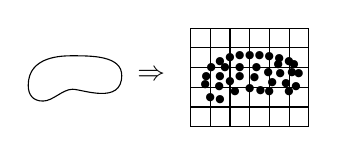
\begin{tikzpicture}[scale=0.25]
  % \draw[step=1.0,black,thin] (-3.,-1.) grid (3,4.);
  % \draw (-3,-1) -- (3,-1) -- (3,4) -- (-3,4) -- (-3,-1);
  \begin{scope}[scale=0.5]
    \draw (-3,0.6) .. controls +(1,0) and +(-1,0) .. (0,1.8)  
    .. controls +(1,0) and +(0,-3) .. (5,3.2) 
    .. controls +(0,2) and +(2,0)  .. (0,5.2) 
    .. controls +(-1,0) and +(0,3) .. (-4.5,2.2) 
    .. controls +(0,-1) and +(-1,0).. (-3,0.6) ;
    \begin{scope}  % pour limiter la portée du clip
      \clip (-3,0.6) .. controls +(1,0) and +(-1,0) .. (0,1.8) 
      .. controls +(1,0) and +(0,-3) .. (5,3.2)
      .. controls +(0,2) and +(2,0)  .. (0,5.2)
      .. controls +(-1,0) and +(0,3) .. (-4.5,2.2)
      .. controls +(0,-1) and +(-1,0).. (-3,0.6);
    \end{scope}
    %\node[below] at (0,1) {$\Omega$};
  \end{scope}
  \node at (4.,1.62) {$\Rightarrow$};
  \begin{scope}[shift={(9,0)}]
    \draw[step=1.0,black,thin] (-3.,-1.) grid (3,4.);
    % contour
    \node at (0,0.9) {\scriptsize$\bullet$}  ;
    \node at (2.5,1.65) {\scriptsize$\bullet$}  ; 
    \node at (0,2.6) {\scriptsize$\bullet$}  ;
    \node at (-2.25,1.1) {\scriptsize$\bullet$}  ; 
    \node at (-1.5,0.35) {\scriptsize$\bullet$}  ; 
    \node at (-2.,0.45) {\scriptsize$\bullet$} ;
    \node at (-2.2,1.5) {\scriptsize$\bullet$}  ; 
    \node at (-1.5,2.3) {\scriptsize$\bullet$} ; 
    \node at (2.35,1.) {\scriptsize$\bullet$}  ;
    \node at (2.25,2.15) {\scriptsize$\bullet$}  ;
    \node at (0.55,0.8) {\scriptsize$\bullet$}  ; 
    \node at (-0.5,2.6) {\scriptsize$\bullet$};
    \node at (0.5,2.59) {\scriptsize$\bullet$}  ;
    \node at (1.5,2.45) {\scriptsize$\bullet$}  ;
    \node at (1,0.75) {\scriptsize$\bullet$}; 
    \node at (2,0.75) {\scriptsize$\bullet$}  ;
    \node at (2,2.3) {\scriptsize$\bullet$}  ;
    \node at (1,2.55) {\scriptsize$\bullet$}  ;
    \node at (-1,2.5) {\scriptsize$\bullet$}  ; 
    \node at (-1.95,2.) {\scriptsize$\bullet$}  ;
    % interior
    \node at (-1.5,1.5) {\scriptsize$\bullet$}  ; 
    \node at (-1.25,2.) {\scriptsize$\bullet$}  ;
    \node at (-0.75,0.75) {\scriptsize$\bullet$}  ; 
    \node at (-1.55,1.){\scriptsize$\bullet$} ;
    \node at (-0.5,1.5) {\scriptsize$\bullet$}  ; 
    \node at (-0.5,2.) {\scriptsize$\bullet$}  ;
    \node at (0.25,1.45) {\scriptsize$\bullet$}  ;
    \node at (0.35,2.) {\scriptsize$\bullet$}  ;
    \node at (0.95,1.75) {\scriptsize$\bullet$}  ;
    \node at (1.15,1.2) {\scriptsize$\bullet$} ;
    \node at (1.45,2.15) {\scriptsize$\bullet$}  ; 
    \node at (1.55,1.65) {\scriptsize$\bullet$}  ;
    \node at (1.85,1.15) {\scriptsize$\bullet$}  ; 
    \node at (2.15,1.75) {\scriptsize$\bullet$}  ;
    \node at (-1.,1.25) {\scriptsize$\bullet$}  ;
    % \draw(3,0.5) -- (3.4,0.5) node [right]  {$\Omega_g$};
  \end{scope}
\end{tikzpicture}

%%% Local Variables:
%%% mode: latex
%%% TeX-master: "../presentation"
%%% End:

  %   %Projection of fields Particles $\Leftrightarrow$ Nodes
  % \end{block}
  \begin{columns}
    \begin{column}{0.4\textwidth}
      \begin{block}{\footnotesize Particle-in-cell mapping \cite{PIC}}
       \begin{tikzpicture}[scale=0.5]
          \tkzKiviatDiagram[lattice=4,
          label style/.append style={font=\scriptsize},radial  style/.style ={->},lattice style/.style ={white,opacity=0}]{CFL,Non-diffusive,Distortion-free,Non-oscillating,High-order}
          \tkzKiviatLine[thick,color = black!50](4,4,4,4,4)
          
          \tkzKiviatLine[thick,color = Yellow,fill= Yellow,opacity=.7](3,1,4,4,3)
        \end{tikzpicture}
      \end{block}
    \end{column}
    \begin{column}{0.4\textwidth}
      \begin{block}{\footnotesize FLuid Implicit Particle mapping \cite{PIC_Nishiguchi}}
        \begin{tikzpicture}[scale=0.5]
          \tkzKiviatDiagram[lattice=4,
          label style/.append style={font=\scriptsize},radial  style/.style ={->},lattice style/.style ={white,opacity=0}]{CFL,Non-diffusive,Distortion-free,Non-oscillating,High-order}
          \tkzKiviatLine[thick,color = black!50](4,4,4,4,4)
          
          \tkzKiviatLine[thick,color = Yellow,fill= Yellow,opacity=.7](3,3,4,1,3)
        \end{tikzpicture}
      \end{block}
    \end{column}
  \end{columns}
  \footnoteCite{Sulsky94,PIC_Nishiguchi,PIC}
\end{frame}

\begin{frame}
  \metroset{block=fill}
  \begin{block}{Objective 1}
    Merge the advantages of FEM, FVM and MPM by means of the DG approximation
  \end{block}
  \metroset{block=transparent}
  \begin{block}{The Discontinuous Galerkin Material Point Method}
    \begin{columns}
      \begin{column}{0.6\textwidth}
        \begin{tikzpicture}[scale=0.5]
          \tkzKiviatDiagram[lattice=4,
          label style/.append style={font=\scriptsize},radial  style/.style ={->},lattice style/.style ={white,opacity=0}]{CFL,Non-diffusive,Distortion-free,Non-oscillating,High-order}
          \tkzKiviatLine[thick,color = black!50](4,4,4,4,4)
          
          \tkzKiviatLine[thick,color = Yellow!70](3,1,4,4,3)
          \tkzKiviatLine[thick,color = Purple!70](1,4,1,4,4)
          \tkzKiviatLine[thick,color = Green,fill= Green,opacity=.7](3,2,4,4,3)
        \end{tikzpicture}
      \end{column}
      \begin{column}{0.4\textwidth}
        \textbf{Ingredients:}
        \begin{itemize}
        \item MPM space discretization
        \item PIC projection of fields
        \item DG approximation
        \end{itemize}
      \end{column}
    \end{columns}
  \end{block}
\end{frame}

\begin{frame}{The simulation is bounded by the model}
  %%
  \begin{block}{Inheritance from fluid dynamics}
    Numerical tools to embed information about the solution in numerical approaches
  \end{block}
  \begin{block}{Point of view adopted}
    \begin{itemize}
    \item Such numerical tools + robust discretization techniques $\rightarrow$ accurate solutions
    \item Make a numerical approach able to mimic the physical response
    \end{itemize}
  \end{block}
  \begin{block}{Limitations}
    Gaps about some constitutive models (damage, plasticity, thermo-mechanical coupling etc.)
  \end{block}
  \metroset{block=fill}
  \begin{block}{Objective 2}
    Investigate the response of two-dimensional elastic-plastic solids to dynamic loading
  \end{block}
\end{frame}



%%% Local Variables:
%%% mode: latex
%%% TeX-master: "../presentation"
%%% End:
